\documentclass{standalone}

\usepackage{amsmath}
\usepackage{tikz}
\usetikzlibrary{arrows.meta, positioning, calc}

% Respect chosen fonts (serif) and metrics
\renewcommand{\familydefault}{\rmdefault}

%% font
\usepackage{dsfont}
\usepackage[T1]{fontenc}
\usepackage{lmodern}
\usepackage{amsmath}

\begin{document}

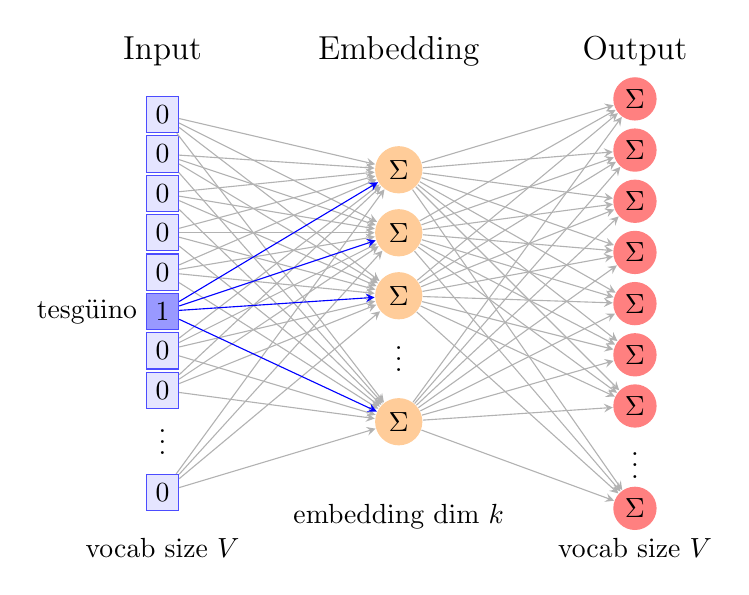
\begin{tikzpicture}[
    >=stealth,
    inputnode/.style={rectangle, draw=blue!70, fill=blue!10, minimum width=3.5mm, minimum height=3.5mm},
    hiddennode/.style={circle, fill=orange!40, minimum size=6mm, inner sep=0pt},
    outputnode/.style={circle, fill=red!50, minimum size=5.5mm, inner sep=0pt},
    conn/.style={gray!60,->,thin}
]

% X positions
\def\xin{0}
\def\xhid{3}
\def\xout{6}

% Y grid (shared across layers)
\def\yA{4.5}
\def\yB{4.0}
\def\yC{3.5}
\def\yD{3.0}
\def\yE{2.5}
\def\yF{2.0}
\def\yG{1.5}
\def\yH{1.0}
\def\yI{0.5}

% ---------- Titles ----------
\node[font=\large] at (\xin,5.3) {Input};
\node[font=\large] at (\xhid,5.3) {Embedding};
\node[font=\large] at (\xout,5.3) {Output};

% ---------- Input ----------
\node[inputnode] (I1) at (\xin,\yA) {0};
\node[inputnode] (I2) at (\xin,\yB) {0};
\node[inputnode] (I3) at (\xin,\yC) {0};
\node[inputnode] (I4) at (\xin,\yD) {0};
\node[inputnode] (I5) at (\xin,\yE) {0};

\node[inputnode, fill=blue!40] (Istar) at (\xin,\yF) {1};

\node[inputnode] (I6) at (\xin,\yG) {0};
\node[inputnode] (I7) at (\xin,\yH) {0};

\node at (\xin,0.45) {$\vdots$};
\node[inputnode] (Ilast) at (\xin,-0.3) {0};

% label
\node[left] at (-0.2,\yF) {tesg\"uino};
\node at (\xin,-1.0) {vocab size $V$};

% ---------- Hidden ----------
\node[hiddennode] (H1) at (\xhid,3.8) {$\Sigma$};
\node[hiddennode] (H2) at (\xhid,3.0) {$\Sigma$};
\node[hiddennode] (H3) at (\xhid,2.2) {$\Sigma$};

\node at (\xhid,1.5) {$\vdots$};

\node[hiddennode] (Hk) at (\xhid,0.6) {$\Sigma$};

\node at (\xhid,-0.6) {embedding dim $k$};

% ---------- Output (evenly spaced, WORKING VERSION) ----------
\def\dy{0.65}
\def\ytop{4.7}
\def\nout{7}

% visible nodes
\foreach \i in {1,...,\nout} {
    \pgfmathsetmacro{\y}{\ytop - (\i-1)*\dy}
    \node[outputnode] (O\i) at (\xout,\y) {$\Sigma$};
}

% dots
\pgfmathsetmacro{\ydots}{\ytop - \nout*\dy}
\node at (\xout,\ydots) {$\vdots$};

% last node
\pgfmathsetmacro{\ylast}{\ytop - (\nout+1)*\dy}
\node[outputnode] (Olast) at (\xout,\ylast) {$\Sigma$};

\node at (\xout,-1.0) {vocab size $V$};

% ---------- Connections (from active input only) ----------
% Connections: ALL inputs -> hidden
\foreach \i in {I1,I2,I3,I4,I5,I6,I7,Ilast}
    \foreach \h in {H1,H2,H3,Hk}
        \draw[conn] (\i) -- (\h);

\foreach \i in {Istar}
    \foreach \h in {H1,H2,H3,Hk}
        \draw[conn,color=blue] (\i) -- (\h);
        
\foreach \h in {H1,H2,H3,Hk}
    \foreach \o in {O1,O2,O3,O4,O5,O6,O7,Olast}
        \draw[conn] (\h) -- (\o);

\end{tikzpicture}

\end{document}